

\chapter{Results and Discussion}
\label{results}
This thesis basically defines $5$ new methods: $2$ single model-based and $3$ clustering-based. For each of them, features from QMEAN are considered as input. It is important to highlight that the new implemented clustering algorithm does not depend on a QMEAN-based method, but could use a generic MQAP as support to weight model scores. Trying other MQAPs as support methods may be an interesting test to do in the near future with the intent to further outperform the reported results.
The main descriptions of the methods proposed are the following:
\begin{description}
	\item[QMEANrannZ:] The final model score is achieved by a single raw neural network.
	\item[QMEANeannZ:] The target model scores of QMEANrannZ are used to classify the relative target in the FM, TBM or HQM classes. Then, the target models are scored by an expert neural network, associated to that category.
	\item[QMEANrannclustZ:] The implemented clustering algorithm uses QMEANrannZ as support MQAP.
	\item[QMEANeannclustZ:] The implemented clustering algorithm uses QMEAN\-eannZ as support MQAP.
	\item[QMEANclustZ:] The implemented clustering algorithm uses QMEAN as support MQAP.
\end{description}

The reported results distinguish whether the used ANNs have a fixed or a ca\-sca\-de-\-cor\-re\-la\-tion architecture.\\
In addition to the above methods, experiments also involve new features aside from those standard for QMEAN, such as Gauss integrals, hydrogen bonds and TAP score (see \S~\ref{subsec:addition_of_new_features}). Therefore, depending on the features utilized, the following different schemes are proposed:
\begin{description}
\item[std\_median] All ANNs use only features from QMEAN (neural networks with $6$ input units).
\item[std\_G\_median] All ANNs use features from QMEAN and GIT (neural networks with $13$ input units).
\item[std\_H\_median] All ANNs use features from QMEAN and HBPLUS (neural networks with $7$ input units).
\item[std\_GH\_median] All ANNs use features from QMEAN, GIT and HBPLUS (neural networks with $14$ input units).
\item[std\_3n\_T\_median] All ANNs are identical to the scheme \emph{std\_median} (``n'' stands for no-addition), except the HQM expert ANN that uses also the TAP score feature (neural networks with $6$ input units, whereas HQM expert ANN with $7$ input units).
\item[std\_3H\_HT\_median] All ANNs are identical to the scheme \\\emph{std\_H\_median}, except the HQM expert ANN that uses also the TAP score feature (neural networks with $7$ input units, whereas HQM expert ANN with $8$ input units).
\item[std\_3GH\_GHT\_median] All ANNs are identical to the scheme \emph{std\_GH\_\-median}, except the HQM expert ANN that uses also the TAP score  feature (neural networks with $14$ input units, whereas HQM expert ANN with $15$ input units).
\end{description}
Every scheme contains the substring \emph{median} because the target categorization uses the median to classify targets (see \S~\ref{subsec:target_categorization}). The sub-string \emph{std} means that the standard QMEAN features are included. The letters G, H and T define if features from GIT, HBPLUS and TAP score are inserted. The last three schemes, \emph{std\_3n\_T\_median}, \emph{std\_3H\_HT\_median} and \emph{std\_3GH\_GHT\_\-median}, consider different architectures for the components of the neural system. Four groups of letters specify the features used respectively for the Raw, FM, TBM and HQM neural networks. In the proposed schemes, the number $3$ is used to simplify the notation by collecting the first three groups in one.

\section{Artificial Neural Network Training}
\label{sec:ann_training}
In this work, ANNs are trained and validated using data from CASP-5, CASP-6 and CASP-7 (214 targets for a total of 78,854 models). Only the ANN training from the scheme \emph{std\_H\_median} is shown because this scheme obtains the best results (see Table \ref{tab:casp8_comparison}). Training for the other schemes provides substantially similar results to these and is omitted for this reason. For this scheme and for both fixed and variable topology ANNs, the Raw\_ANN uses all $214$ targets as training and validation sets. The FM\_ANN, TBM\_ANN and HQM\_ANN use $109$, $87$ and $18$ targets respectively. Every point in the scatter plots illustrated in this section represents the average MSE over $5$ MSEs computed during the $5$-fold cross validation. The average MSE is calculated using the formula described in \S~\ref{subsubsec:validation}. \\
For fixed topology ANNs, the training aims to find out the best values for the number of epochs and hidden units. While all the other parameters were held at default value, the number of epochs is chosen in the range $[1, 5000]$ with step size $250$. The increment used to vary the number of epochs is chosen a little large due to the training set width and the number of proposed schemes. A more accurate step size is possible, but is expensive from a computational point of view. Beyond $4500$-$5000$ epochs the ANNs developed in this work tend to overfit. The number of hidden units is taken into account in the range $[2, 5]$ with step size $1$. Figures \ref{fig:raw_ann_validation_error_epochs} - \ref{fig:hqm_ann_validation_error_epochs} show the validation set errors with respect to the number of epochs for Raw\_ANN, FM\_ANN, TBM\_ANN and HQM\_ANN respectively. In the legend, the label called AVG\_MSE\_$n$HU distinguishes the number of hidden units ($n$) that has been used. 
The optimized numbers of epochs and hidden units are $(4500, 3)$, $(4000, 4)$, $(3000, 5)$ and $(1500, 2)$ for Raw\_ANN, FM\_ANN, TBM\_ANN and HQM\_ANN respectively.\\
For ca\-sca\-de-\-cor\-re\-la\-tion ANNs, only the number of hidden units is considered in the range $[1, 25]$ with step size $1$. For this type of architecture, the number of epochs is optimized during the training phase by the ca\-sca\-de-\-cor\-re\-la\-tion algorithm. Figures \ref{fig:raw_ann_validation_error_hu} - \ref{fig:hqm_ann_validation_error_hu} show the validation set errors with respect to the number of hidden units for the Raw\_ANN, FM\_ANN, TBM\_ANN and HQM\_ANN respectively. Increasing the number of hidden units has two important consequences. First, the computed average MSE quickly increases or decreases for each added hidden unit. Second, it produces overfitted ANNs. For these reasons it is better to consider the number of hidden units as low as possible. The optimized numbers of hidden units are of $9$, $8$, $8$ and $5$ for Raw\_ANN, FM\_ANN, TBM\_ANN and HQM\_ANN respectively.

\begin{figure}[H]
	\begin{center}
		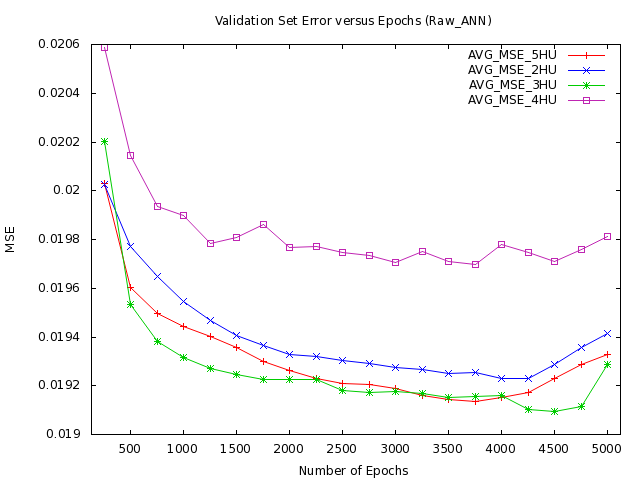
\includegraphics[scale=0.50]{raw_ann_validation_error_epochs}
		\caption[Validation set error versus number of epochs for Raw\_ANN using fixed architecture]{Validation set error versus number of epochs for Raw\_ANN using a fixed architecture. The lower MSE is reached by using 3 hidden units and training for $4500$ epochs.}
		\label{fig:raw_ann_validation_error_epochs}
	\end{center}
\end{figure}
\begin{figure}[H]
	\begin{center}
		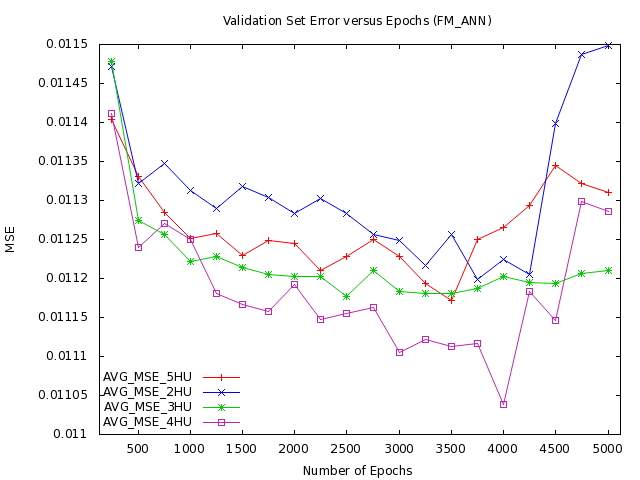
\includegraphics[scale=0.50]{fm_ann_validation_error_epochs}
		\caption[Validation set error versus number of epochs for FM\_ANN using fixed architecture]{Validation set error versus number of epochs for FM\_ANN using a fixed architecture. The lower MSE is reached by using 4 hidden units and training for $4000$ epochs.}
		\label{fig:fm_ann_validation_error_epochs}
	\end{center}
\end{figure}
\begin{figure}[H]
	\begin{center}
		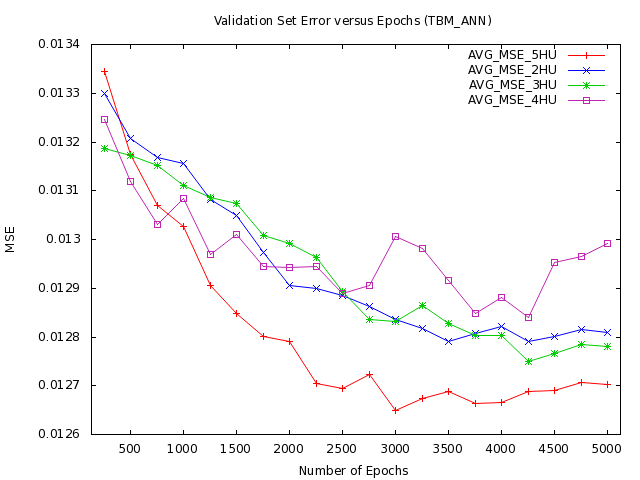
\includegraphics[scale=0.50]{tbm_ann_validation_error_epochs}
		\caption[Validation set error versus number of epochs for TBM\_ANN using fixed architecture]{Validation set error versus number of epochs for TBM\_ANN using a fixed architecture. The lower MSE is reached by using 5 hidden units and training for $3000$ epochs.}
		\label{fig:tbm_ann_validation_error_epochs}
	\end{center}
\end{figure}
\begin{figure}[H]
	\begin{center}
		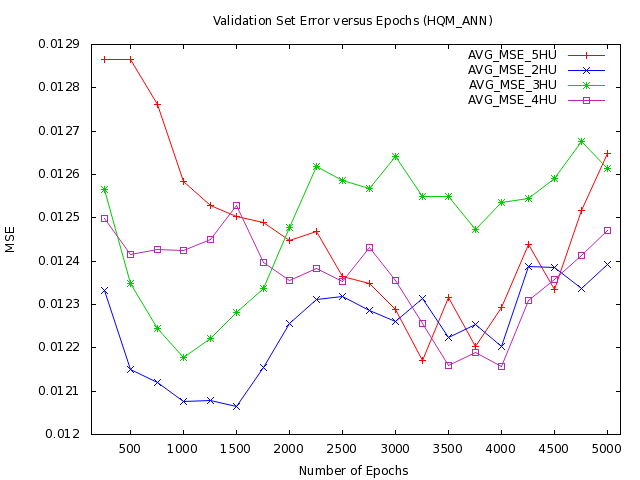
\includegraphics[scale=0.50]{hqm_ann_validation_error_epochs}
		\caption[Validation set error versus number of epochs for HQM\_ANN using fixed architecture]{Validation set error versus number of epochs for HQM\_ANN using a fixed architecture. The lower MSE is reached by using 2 hidden units and training for $1500$ epochs.}
		\label{fig:hqm_ann_validation_error_epochs}
	\end{center}
\end{figure}


\begin{figure}[H]
	\begin{center}
		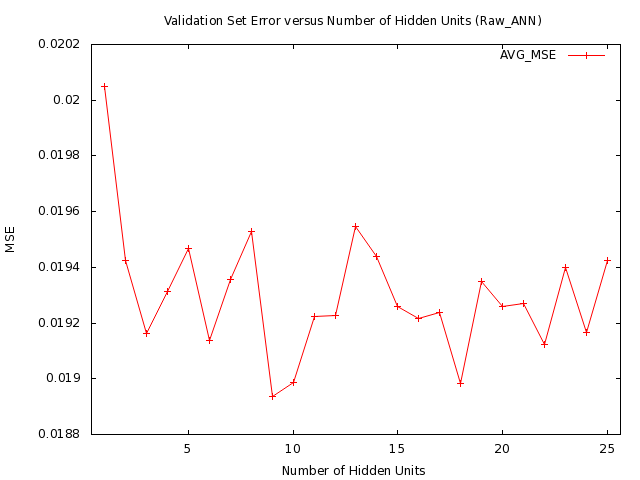
\includegraphics[scale=0.50]{raw_ann_validation_error_hu}
		\caption[Validation set error versus number of hidden units for Raw\_ANN using ca\-sca\-de-\-cor\-re\-la\-tion architecture]{Validation set error versus number of hidden units for Raw\_ANN using ca\-sca\-de-\-cor\-re\-la\-tion architecture. The lower MSE is reached by using 9 hidden units.}
		\label{fig:raw_ann_validation_error_hu}
	\end{center}
\end{figure}
\begin{figure}[H]
	\begin{center}
		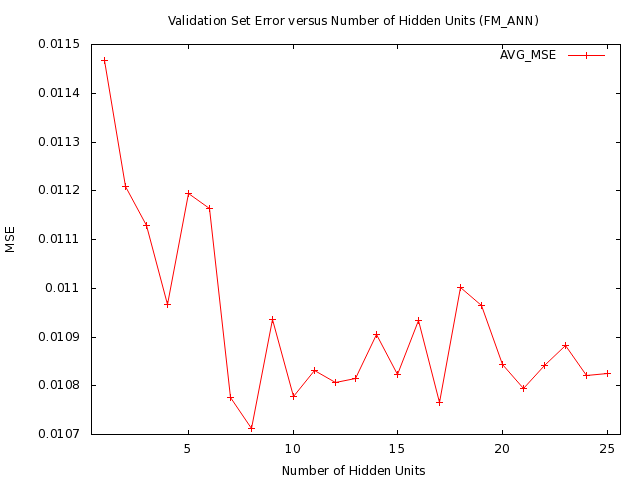
\includegraphics[scale=0.50]{fm_ann_validation_error_hu}
		\caption[Validation set error versus number of hidden units for FM\_ANN using ca\-sca\-de-\-cor\-re\-la\-tion architecture]{Validation set error versus number of hidden units for FM\_ANN using ca\-sca\-de-\-cor\-re\-la\-tion architecture. The lower MSE is reached by using 8 hidden units.}
		\label{fig:fm_ann_validation_error_hu}
	\end{center}
\end{figure}
\begin{figure}[H]
	\begin{center}
		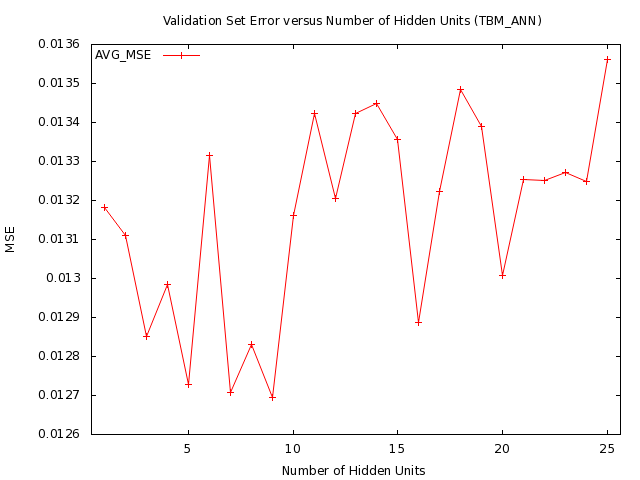
\includegraphics[scale=0.50]{tbm_ann_validation_error_hu}
		\caption[Validation set error versus number of hidden units for TBM\_ANN using ca\-sca\-de-\-cor\-re\-la\-tion architecture]{Validation set error versus number of hidden units for TBM\_ANN using ca\-sca\-de-\-cor\-re\-la\-tion architecture. The lower MSE is reached by using 8 hidden units.}
		\label{fig:tbm_ann_validation_error_hu}
	\end{center}
\end{figure}
\begin{figure}[H]
	\begin{center}
		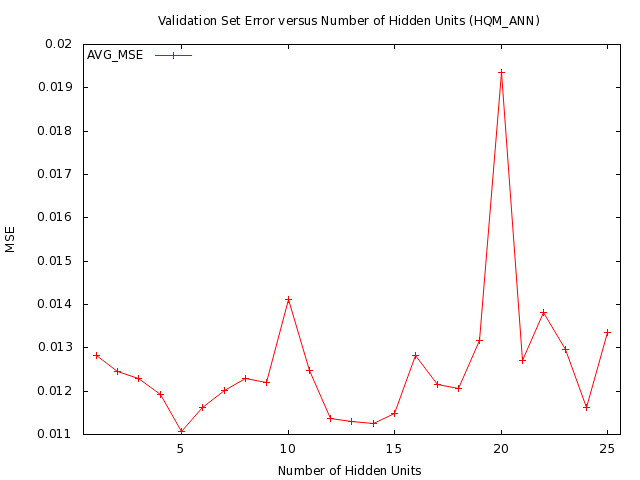
\includegraphics[scale=0.50]{hqm_ann_validation_error_hu}
		\caption[Validation set error versus number of hidden units for HQM\_ANN using ca\-sca\-de-\-cor\-re\-la\-tion architecture]{Validation set error versus number of hidden units for HQM\_ANN using ca\-sca\-de-\-cor\-re\-la\-tion architecture. The lower MSE is reached by using 5 hidden units.}
		\label{fig:hqm_ann_validation_error_hu}
	\end{center}
\end{figure}



\section{Clustering Optimizations}
\label{sec:clustering_optimization}

\subsection{Semi-Clustering Optimization}
\label{subsec:semiclustering_optimization}
In this section, the optimization of the best percentages for FM, TBM and HQM targets is provided by considering data from CASP-5, CASP-6 and CASP-7. These percentages serve to extract from all target models a subset of the best structures which will be used in the clustering procedure. \\
QMEAN is used in this optimization due to reduce problems related to overfitting. In fact, the QMEAN weight vector is optimized only on data from CASP-6. Being trained on the same data, the individual methods developed in this work obviously cannot be used in this procedure because they would provide an overestimation (see \S~\ref{subsec:training_and_testing_phases}). Discarding data from CASP-6, the final clustering accuracy substantially worsens using, as support MQAP, any implemented individual method or QMEAN itself. This fact could be explained with the lack of several models (in particular high quality models which are not frequent).\\
The optimization plots for FM, TBM and HQM targets are shown in Figures \ref{fig:thresholdFM} - \ref{fig:thresholdHQM} respectively. For FM targets, the best computed percentage is $93\%$ which achieves a Pearson correlation of $0.9036$. For TMB targets, the best percentage is $93\%$ obtaining $0.9617$ of Pearson correlation. Finally, for HQM targets, the best percentage is $85\%$ achieving a Pearson correlation of $0.9985$.
\begin{figure}[htbp]
	\begin{center}
		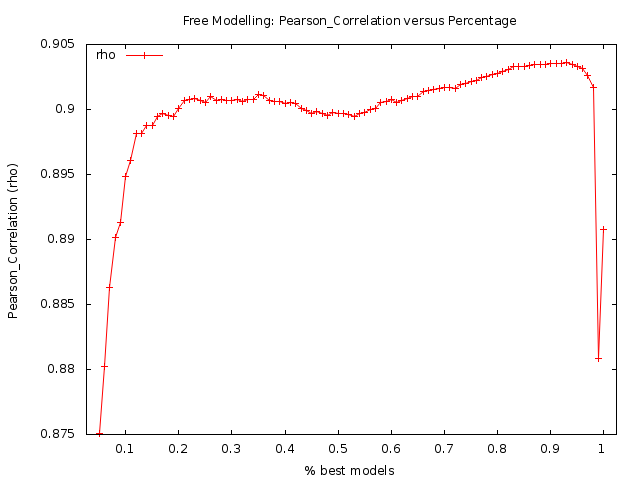
\includegraphics[scale=0.50]{thresholdFM}
		\caption[Optimization of the best percentage for FM targets]{Optimization of the best percentage for FM targets in CASP-5, CASP-6 and CASP-7. The highest Pearson correlation is $0.9036$, obtained by using $93\%$ of the best models.}
		\label{fig:thresholdFM}
	\end{center}
\end{figure}
\begin{figure}[htbp]
	\begin{center}
		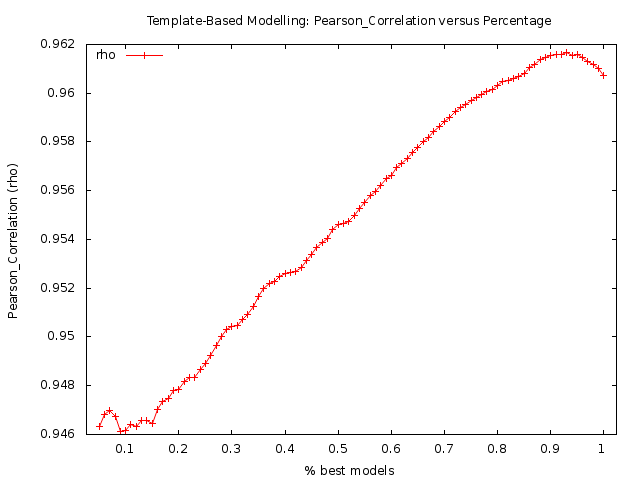
\includegraphics[scale=0.50]{thresholdTBM}
		\caption[Optimization of the best percentage for TBM targets]{Optimization of the best percentage for TBM targets in CASP-5, CASP-6 and CASP-7. The highest Pearson correlation is $0.9617$, obtained by using $93\%$ of the best models.}
		\label{fig:thresholdTBM}
	\end{center}
\end{figure}
\begin{figure}[htbp]
	\begin{center}
		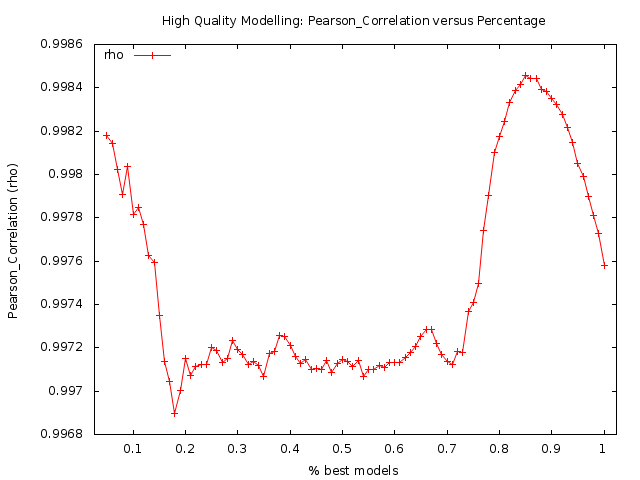
\includegraphics[scale=0.50]{thresholdHQM}
		\caption[Optimization of the best percentage for HQM targets]{Optimization of the best percentage for HQM targets in CASP-5, CASP-6 and CASP-7. The highest Pearson correlation is $0.9985$, obtained by using $85\%$ of the best models.}
		\label{fig:thresholdHQM}
	\end{center}
\end{figure}


\subsection{Parabolic Fraction Modelled}
\label{subsec:parabolic_fraction_modelled}
Table \ref{tab:fraction_modelled_functions} shows the improvement gained by using the $PFractionModelled$ feature with respect to the standard $FractionModelled$. The Pearson correlation is adopted in order to evaluate the performance of this optimization. Data from CASP-4 and CASP-8 are used as comparison. To illustrate the improvement, QMEAN is chosen as support MQAP to the implemented clustering-based method. On the other hand, usage of the developed individual methods in place of QMEAN, as support MQAP, has reported the same results and, for this reason, the latter are omitted. The $PFractionModelled$ represents a significative improvement with respect to the $FractionModelled$ of $\approx 0.5\%$ in CASP-8, reducing also the presence of false positives without penalizing HQM scores. In the same dataset the $PFractionModelled$ improves the clustering algorithm of $\approx 0.8\%$ with respect to the same algorithm which does not consider any $FractionModelled$-like function.
\begin{table}[H]
\center
\begin{tabular}{lcc}
\toprule                % or \hline
\textbf{QMEANclustZ}	&\textbf{CASP-4}	&\textbf{CASP-8}\\
\midrule                % or \hline
	No $FractionModelled$	&0.9408	&0.9392\\
	$FractionModelled$	&0.9468	&0.9420\\
	$PFractionModelled$	&0.9477	&0.9473\\
\bottomrule               % or \hline
\end{tabular}
\caption[Different fraction modelled evaluation]{Pearson correlation achieved in the CASP-4 and CASP-8 test sets by QMEANclustZ configured with different fraction modelled functions. QMEANclustZ with the $FractionModelled$ feature outperforms QMEANclustZ without the use of the feature. However the application of the pure $FractionModelled$ feature often reduces  too much model scores. QMEANclustZ with the $PFractionModelled$ feature outperforms significatively all the other variants proposed.}
\label{tab:fraction_modelled_functions}
\end{table}


\clearpage

\section{Performance on the CASP-4 and CASP-8 Datasets}
This section aims to illustrate the results achieved from the clustering-based and individual methods developed in this work. Results are presented and discussed by considering two different test sets: CASP-4 and CASP-8 (see \S~\ref{subsec:training_and_testing_phases}). The latter is more important because it contains more targets and is built by keeping in mind the aim of the MQAP category at CASP. Thus, the CASP-4 test set serves to confirm the reliability of the implemented methods. For each scheme, both Pearson and Spearman correlations are used with the intent to gain more reliable and accurate results. \\
For the CASP-8 test set, a comparison against the best $9$ MQAPs that participated to the CASP-8 experiment is presented. These methods are currently the best of the world. Scores computed by these MQAPs are retrieved from the CASP web page.\\
For the CASP-4 test set, only the QMEAN scores are reported as comparison against an external method because QMEAN is the only MQAP completely available in the laboratory where this work has been developed and no data is available from the CASP website.\\
The feature extracted from the program TAPscore is shown to decrease the accuracy of the method when used. The reason could be associated to the use of protein models instead of experimental structures. Although this feature is adopted only for HQM models, which are models very similar to the native structure, the TAPscore program often returns a score of $0$ for certain target models. This fact could mislead the HQM\_ANN prediction.\\
The following sections present and discuss the performance achieved on the CASP-4 and CASP-8 test sets.


\subsection{Performance on the CASP-4 Dataset}
\label{subsec:performance_on_the_casp4_dataset}
Tables \ref{tab:casp4} and \ref{tab:casp4_cascade} report the performances achieved by using fixed and ca\-sca\-de-\-cor\-re\-la\-tion ANN architectures, respectively. Methods are not directly comparable because the initial neural networks are different due to the different number of input units occuring among schemes. However, by considering both Pearson and Spearman correlations a higher reliability and accuracy of methods could be achieved. The schemes \emph{std\_median} and \emph{std\_H\_median} report more reliable and higher accuracy results with respect to the other schemes. Figure \ref{fig:casp4_qmean} reports the QMEAN versus GDT\_TS scatter plot. Figure \ref{fig:casp4_qmeanclustZ} shows the accuracy of the clustering implemented in this work using QMEAN as support MQAP. Figures \ref{fig:casp4_std_H_medianQMEANrannclustZ} - \ref{fig:casp4_std_medianQMEANeannZ} illustrate the best scatter plots achieved by methods based on fixed ANN architectures. Figures \ref{fig:casp4_cascade_std_H_medianQMEANeannclustZ} - \ref{fig:casp4_cascade_std_medianQMEANrannclustZ} show the best scatter plots obtained by methods based on ca\-sca\-de-\-cor\-re\-la\-tion ANN architectures. \\
For fixed topology ANNs, the scheme \emph{std\_H\_median} substantially obtains the best correlations for both the individual and the clustering-based methods. The achieved best Pearson correlations are $0.8799$ and $0.9485$ for QMEANeannZ (scheme \emph{std\_median}) and QMEANeannclustZ (scheme \emph{std\_H\_median}) respectively. The gained best Spearman correlations are $0.7278$ and $0.9513$ for QMEANrannZ (scheme \emph{std\_H\_median}) and QMEANrannclustZ (scheme \emph{std\_H\_median}) respectively.\\
For ca\-sca\-de-\-cor\-re\-la\-tion ANNs, the best results are more accurate than those achieved using fixed topology ANNs. The best schemes are \emph{std\_median} and \emph{std\_H\_median}. QMEANeannZ (scheme \emph{std\_median}) and QMEANeannclustZ (scheme \emph{std\_H\_median}) achieve the best Pearson correlations of $0.8901$ and $0.9489$ respectively. On the other hand, QMEANeannZ (scheme \emph{std\_H\_median}) and QMEANrannclustZ (scheme \emph{std\_median}) gain the best Spearman correlations of $0.7601$ and $0.9515$ respectively. 
For both the architectures, almost all proposed individual methods outperform significatively QMEAN which achieves $0.7844$ and $0.7102$ of Pearson and Spearman correlations respectively.


\begin{table}[htbp]
\center
\begin{tabular}{lcc}
\toprule                % or \hline
\textbf{Method Variants} & \textbf{Pearson} & \textbf{Spearman} \\
	\midrule                % or \hline
	\emph{\textbf{std\_median}} & &\\
	QMEANrannZ	&0.8264	&0.7126\\
	QMEANeannZ	&\textbf{0.8799}	&0.7060\\
	QMEANrannclustZ	&0.9461	&0.9499\\
	QMEANeannclustZ	&0.9479	&0.9493\\
	\midrule                % or \hline	
	\emph{\textbf{std\_G\_median}}	 & &\\
	QMEANrannZ	&0.8448	&0.7262\\
	QMEANeannZ	&0.7664	&0.6681\\
	QMEANrannclustZ	&0.9468	&0.9504\\
	QMEANeannclustZ	&0.9471	&0.9467\\
	\midrule                % or \hline	
	\emph{\textbf{std\_H\_median}}	& &\\
	QMEANrannZ	&0.8346	&\textbf{0.7278}\\
	QMEANeannZ	&0.8798	&0.7237\\
	QMEANrannclustZ	&0.9463	&\textbf{0.9513}\\
	QMEANeannclustZ	&\textbf{0.9485}	&0.9499\\	
	\midrule                % or \hline	
	\emph{\textbf{std\_GH\_median}}	& &\\
	QMEANrannZ	&0.8340	&0.7102\\
	QMEANeannZ	&0.8390	&0.7061\\
	QMEANrannclustZ	&0.9456	&0.9498\\
	QMEANeannclustZ	&0.9471	&0.9473\\	
	\midrule                % or \hline	
	\emph{\textbf{std\_3n\_T\_median}}	& &\\
	QMEANeannZ	&0.8301	&0.7065\\
	QMEANeannclustZ	&0.9478	&0.9492\\	
	\midrule                % or \hline	
	\emph{\textbf{std\_3H\_HT\_median}}	& &\\
	QMEANeannZ	&0.8473	&0.7065\\
	QMEANeannclustZ	&0.9483	&0.9493\\		
	\midrule                % or \hline	
	\emph{\textbf{std\_3GH\_GHT\_median}}	& &\\
	QMEANeannZ	&0.8389	&0.7061\\
	QMEANeannclustZ	&0.9470	&0.9472\\
	\midrule                % or \hline
	\emph{\textbf{Clustering using QMEAN}} & &\\
	QMEANclustZ	&0.9477	&0.9448\\	
	\midrule                % or \hline	
	\emph{\textbf{External MQAPs}} & &\\	
	QMEAN	&0.7844	&0.7102\\
\bottomrule                % or \hline
\end{tabular}
\caption[Performance on the CASP-4 test set using neural networks based on fixed ANN architecture]{Correlation on the CASP-4 test set using neural networks based on fixed ANN architecture. The best results are shown in bold face (for Pearson and Spearman correlations, for individual and clustering-based methods). The scheme \emph{std\_H\_median} obtains the best correlation for both the individual and the clustering-based methods. All individual proposed methods outperform significatively QMEAN, except QMEANeannZ with Gauss integrals. All clustering-based methods that use ANNs as support MQAP show an improved Spearman correlation with respect to the same clustering that uses QMEAN as support MQAP.}
\label{tab:casp4}
\end{table}


\begin{table}[htbp]
\center
\begin{tabular}{lcc}
\toprule                % or \hline
\textbf{Method Variants} & \textbf{Pearson} & \textbf{Spearman} \\
	\midrule                % or \hline
	\emph{\textbf{std\_median}}	& & \\
	QMEANrannZ	&0.8364	&0.7189\\
 	QMEANeannZ	&\textbf{0.8901}	&0.7325\\
 	QMEANrannclustZ	&0.9469	&\textbf{0.9515}\\
 	QMEANeannclustZ	&0.9484	&0.9493\\
	\midrule                % or \hline
	\emph{\textbf{std\_G\_median}}	 & &\\
	QMEANrannZ	&0.8295	&0.6837\\
 	QMEANeannZ	&0.7997	&0.6567\\
 	QMEANrannclustZ	&0.9461	&0.9484\\
 	QMEANeannclustZ	&0.9450	&0.9437\\
	\midrule                % or \hline
	\emph{\textbf{std\_H\_median}} 	& &\\
	QMEANrannZ	&0.8341	&0.7433\\
 	QMEANeannZ	&0.8844	&\textbf{0.7601}\\
 	QMEANrannclustZ	&0.9471	&0.9505\\
 	QMEANeannclustZ	&\textbf{0.9489}	&0.9510\\
	\midrule                % or \hline
	\emph{\textbf{std\_GH\_median}}	& &\\
	QMEANrannZ	&0.7818	&0.6847\\
 	QMEANeannZ	&0.8270	&0.7149\\
 	QMEANrannclustZ	&0.9461	&0.9481\\
 	QMEANeannclustZ	&0.9470	&0.9491\\
	\midrule                % or \hline
	\emph{\textbf{std\_3n\_T\_median}}	& &\\
 	QMEANeannZ	&0.8300	&0.7313\\
 	QMEANeannclustZ	&0.9482	&0.9493\\
	\midrule                % or \hline	
	\emph{\textbf{std\_3H\_HT\_median}}	& &\\
	QMEANeannZ	&0.8343	&0.7072\\
	QMEANeannclustZ	&0.9486	&0.9499\\		
	\midrule                % or \hline
	\emph{\textbf{std\_3GH\_GHT\_median}}	& &\\
 	QMEANeannZ	&0.8290	&0.7166\\
 	QMEANeannclustZ	&0.9472	&0.9492\\
	\midrule                % or \hline
	\emph{\textbf{Clustering using QMEAN}} & &\\
	QMEANclustZ	&0.9477	&0.9448\\		
	\midrule                % or \hline
	\emph{\textbf{External MQAPs}}	& &\\
	QMEAN	&0.7844	&0.7102\\
\bottomrule                % or \hline
\end{tabular}
\caption[Performance on the CASP-4 test set using neural networks based on ca\-sca\-de-\-cor\-re\-la\-tion ANN architecture]{Correlation on the CASP-4 using neural networks based on ca\-sca\-de-\-cor\-re\-la\-tion ANN architecture. The best results are shown in bold face (for Pearson and Spearman correlations, for individual and clustering-based methods). By using the ca\-sca\-de-\-cor\-re\-la\-tion algorithm, the Spearman correlation is consistent with the growth of the Pearson correlation meaning results more reliable. The best results are also highter than those reported in the corrisponding Table \ref{tab:casp4}, which again could mean that the ca\-sca\-de-\-cor\-re\-la\-tion architecture is more accurate than the fixed one. Almost all proposed individual methods outperform significatively QMEAN. QMEANeannZ using Gauss integrals shows only a low increment of accuracy against QMEAN.}
\label{tab:casp4_cascade}
\end{table}


\begin{figure}[H]
	\begin{center}
		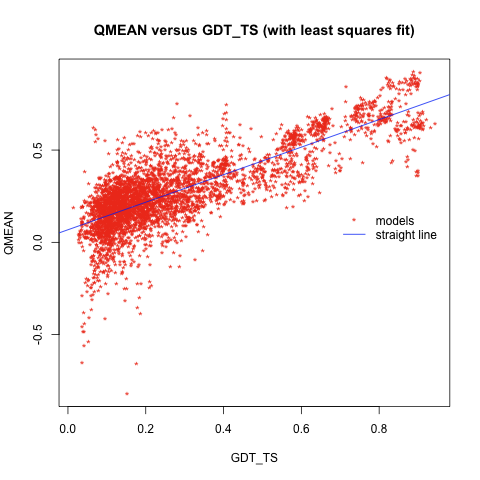
\includegraphics[scale=0.50]{casp4_QMEAN}
		\caption[QMEAN versus GDT\_TS on the CASP-4 test set]{QMEAN versus GDT\_TS on the CASP-4 test set. FM models on the left part of the scatter plot, that receive a negative score by QMEAN, represent obviously method errors.}
		\label{fig:casp4_qmean}
	\end{center}
\end{figure}

\begin{figure}[H]
	\begin{center}
		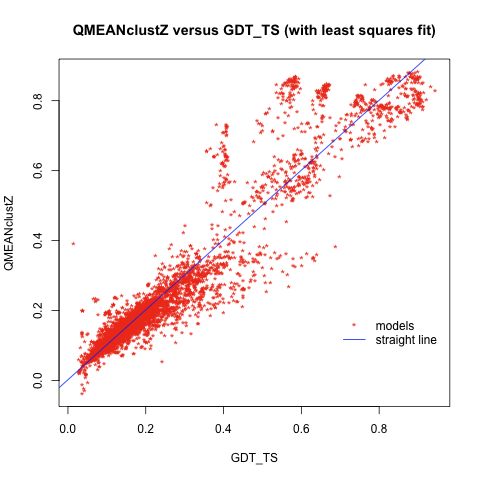
\includegraphics[scale=0.50]{casp4_QMEANclustZ}
		\caption[QMEANclustZ versus GDT\_TS on the CASP-4 test set]{QMEANclustZ versus GDT\_TS on the CASP-4 test set.}
		\label{fig:casp4_qmeanclustZ}
	\end{center}
\end{figure}

\begin{figure}[H]
	\begin{center}
		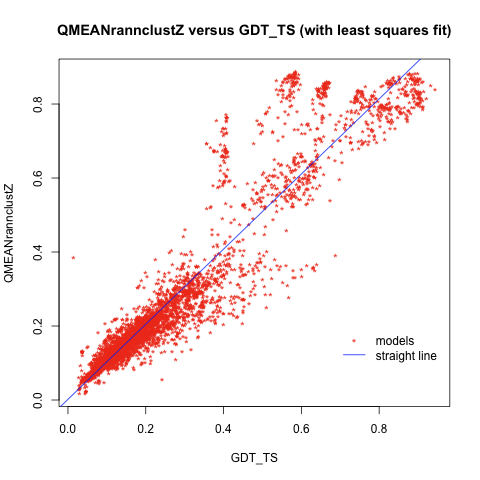
\includegraphics[scale=0.50]{casp4_std_H_medianQMEANrannclustZ}
		\caption[QMEANrannclustZ versus GDT\_TS on the CASP-4 test set, using hydrogen bonds and fixed ANN architecture]{QMEANrannclustZ versus GDT\_TS on the CASP-4 test set, using hydrogen bonds and fixed ANN architecture. A low improvement with respect to Figure \ref{fig:casp4_qmeanclustZ}  is visible on the left-down part of the scatter plot.}
		\label{fig:casp4_std_H_medianQMEANrannclustZ}
	\end{center}
\end{figure}

\begin{figure}[H]
	\begin{center}
		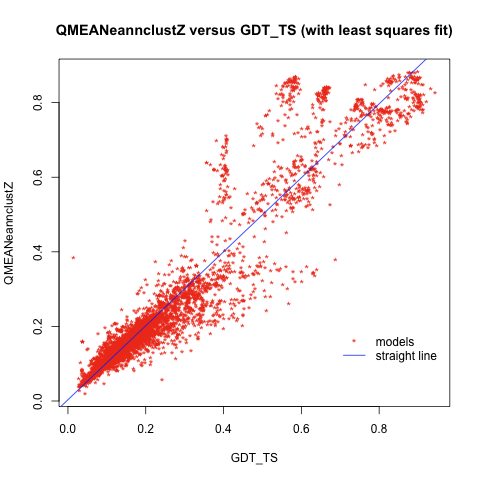
\includegraphics[scale=0.50]{casp4_std_H_medianQMEANeannclustZ}
		\caption[QMEANeannclustZ versus GDT\_TS on the CASP-4 test set, using hydrogen bonds and fixed ANN architectures]{QMEANeannclustZ versus GDT\_TS on the CASP-4 test set, using hydrogen bonds and fixed ANN architectures.}
		\label{fig:casp4_std_H_medianQMEANeannclustZ}
	\end{center}
\end{figure}

\begin{figure}[H]
	\begin{center}
		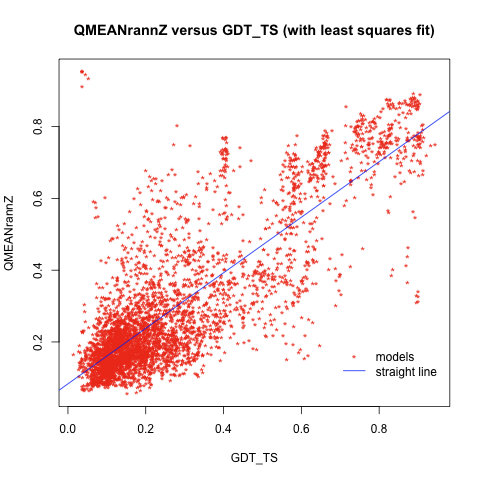
\includegraphics[scale=0.50]{casp4_std_medianQMEANrannZ}
		\caption[QMEANrannZ versus GDT\_TS on the CASP-4 test set, using fixed ANN architecture]{QMEANrannZ versus GDT\_TS on the CASP-4 test set, using fixed ANN architecture. FM scores are more grouped with respect to those given by QMEAN. However, the scatter plot still contains many false positives and negatives.}
		\label{fig:casp4_std_medianQMEANrannZ}
	\end{center}
\end{figure}

\begin{figure}[H]
	\begin{center}
		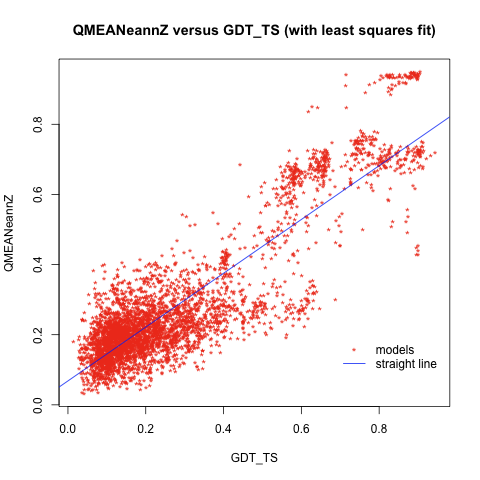
\includegraphics[scale=0.50]{casp4_std_medianQMEANeannZ}
		\caption[QMEANeannZ versus GDT\_TS on the CASP-4 test set, using fixed ANN architectures]{QMEANeannZ versus GDT\_TS on the CASP-4 test set, using fixed ANN architectures. Some false negatives are present on center-bottom of the scatter plot.}
		\label{fig:casp4_std_medianQMEANeannZ}
	\end{center}
\end{figure}

\begin{figure}[H]
	\begin{center}
		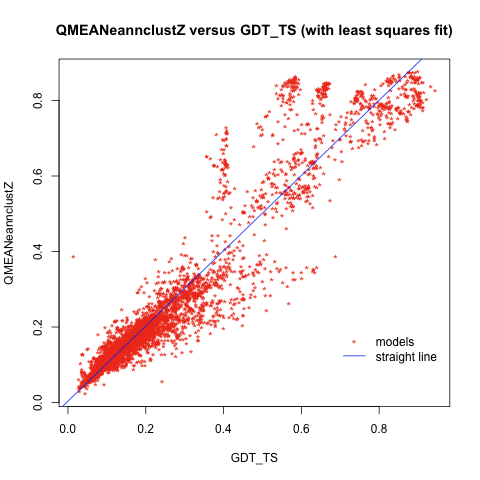
\includegraphics[scale=0.50]{casp4_cascade_std_H_medianQMEANeannclustZ}
		\caption[QMEANeannclustZ versus GDT\_TS on the CASP-4 test set, using hydrogen bonds and ca\-sca\-de-\-cor\-re\-la\-tion ANN architectures]{QMEANeannclustZ versus GDT\_TS on the CASP-4 test set, using hydrogen bonds and ca\-sca\-de-\-cor\-re\-la\-tion ANN architectures.}
	\label{fig:casp4_cascade_std_H_medianQMEANeannclustZ}
	\end{center}
\end{figure}

\begin{figure}[H]
	\begin{center}
		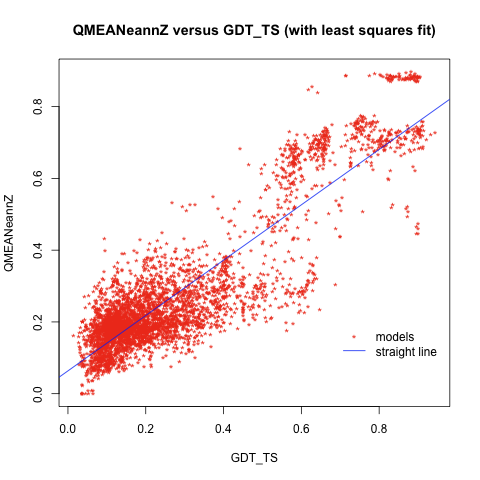
\includegraphics[scale=0.50]{casp4_cascade_std_medianQMEANeannZ}
		\caption[QMEANeannZ versus GDT\_TS on the CASP-4 test set, using ca\-sca\-de-\-cor\-re\-la\-tion ANN architectures]{QMEANeannZ versus GDT\_TS on the CASP-4 test set, using ca\-sca\-de-\-cor\-re\-la\-tion ANN architectures.}
	\label{fig:casp4_cascade_std_medianQMEANeannZ}
	\end{center}
\end{figure}

\begin{figure}[H]
	\begin{center}
		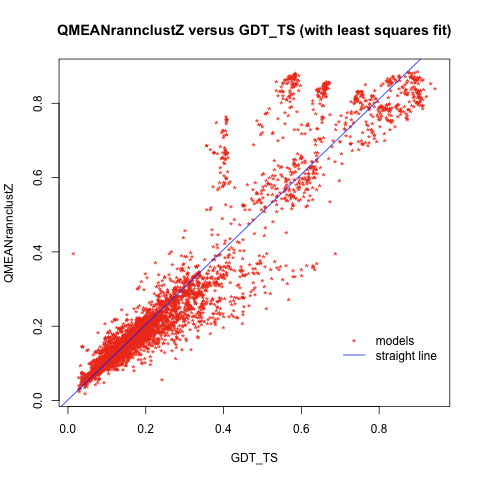
\includegraphics[scale=0.50]{casp4_cascade_std_medianQMEANrannclustZ}
		\caption[QMEANrannclustZ versus GDT\_TS on the CASP-4 test set, using ca\-sca\-de-\-cor\-re\-la\-tion ANN architecture]{QMEANrannclustZ versus GDT\_TS on the CASP-4 test set, using ca\-sca\-de-\-cor\-re\-la\-tion ANN architecture.}
\label{fig:casp4_cascade_std_medianQMEANrannclustZ}
	\end{center}
\end{figure}





\subsection{Performance on the CASP-8 Dataset}
\label{subsec:performance_on_the_casp8_dataset}
The CASP-8 test set is more relevant than the previous one because it contains more selected, difficult and recent protein targets. Tables \ref{tab:casp8} and \ref{tab:casp8_cascade} report the performance obtained respectively by using standard and cascading ANN architectures. The clustering-based methods implemented in this work, outperform significatively all other methods participating at the last CASP-8 experiment, held in December 2008. The best achieved Pearson and Spearman correlations are $0.9485$ and $0.9324$ respectively. The improvement with respect to ModFOLDclust, which is the best participating method and currently the best MQAP of the world, is of $\approx 1\%$ of global Pearson correlation. ModFOLDclust achieves $0.9395$ and $0.9210$ of Pearson and Spearman correlations respectively. All the five best methods achieve a Pearson correlation of $\approx 93\%$. Table \ref{tab:casp8_comparison} shows the comparison against the best $9$ methods plus QMEAN. Using Gauss integrals, methods do not perform well as confirmed in the previous test set, whereas the addition of hydrogen bonds improves the implemented method based solely on QMEAN features. In fact the best evaluated individual and clustering-based methods adopts the hydrogen bonds feature. QMEANclustZ represents an improvement with respect to QMEANclust showing that the clustering algorithm implemented in this work, outperforms the current one. The Pearson and Spearman correlations are $0.9473$ and $0.9309$ for QMEANclustZ, while QMEANclust obtains only $0.9317$ and $0.9199$ respectively. Figures \ref{fig:casp8_qmean} - \ref{fig:casp8_qmeanclustZ} illustrate the scatter plots of QMEAN, QMEANclust and the new QMEANclustZ. Figures \ref{fig:casp8_std_G_median_qmeaneannZ} - \ref{fig:casp8_std_median_qmeanrannZ} represent the most significative scatter plots by using fixed ANN architectures. Figures \ref{fig:casp8_cascade_std_median_qmeanrannZ} - \ref{fig:casp8_cascade_std_H_median_qmeaneannZ} depict the most important scatter plots using ca\-sca\-de-\-cor\-re\-la\-tion ANN architectures. Finally, Figures \ref{fig:casp8_modfoldclust}, \ref{fig:casp8_pcons_pcons} and \ref{fig:casp8_sam-t08-mqac} show the scatter plots of the three best methods participating in CASP-8. The best results are shown in bold face (for Pearson and Spearman correlations, for individual and clustering-based methods).\\
For fixed topology ANNs, the scheme \emph{std\_H\_median} obtains the best correlation for both the individual and the clustering-based methods. The achieved best Pearson correlations are $0.8177$ and $0.9485$ for QMEANeannZ (scheme \emph{std\_H\_median}) and QMEANrannclustZ (scheme \emph{std\_H\_median}) respectively. The gained best Spearman correlations are $0.8151$ and $0.9324$ for the same previously cited method variants respectively.\\
For ca\-sca\-de-\-cor\-re\-la\-tion ANNs, the best results are more accurate than those achieved using fixed topology ANNs. The best schemes are \emph{std\_median} and \emph{std\_H\_median}. QMEANeannZ (scheme \emph{std\_H\_median}) and QMEANrannclustZ (scheme \emph{std\_median}) achieve the best Pearson correlations of $0.8300$ and $0.9482$ respectively. The best Spearman correlations are $0.8237$ and $0.9321$ obtained by the same previously cited method variants respectively. 
For both the architectures, almost all proposed individual methods outperform significatively QMEAN which achieves $0.7651$ and $0.7655$ of Pearson and Spearman correlations respectively.



\begin{table}[htbp]
\center
\begin{tabular}{lcc}
\toprule                % or \hline
\textbf{Method Variants} & \textbf{Pearson} & \textbf{Spearman} \\
	\midrule                % or \hline
	\emph{\textbf{std\_median}}	& &\\
	QMEANrannZ	&0.7817	&0.7786\\
	QMEANeannZ	&0.7888	&0.7834\\
	QMEANrannclustZ	&0.9484	&0.9324\\
	QMEANeannclustZ	&0.9480	&0.9312\\
	\midrule                % or \hline	
	\emph{\textbf{std\_G\_median}} 	& &\\
	QMEANrannZ	&0.7750	&0.7826\\
	QMEANeannZ	&0.6671	&0.7386\\
	QMEANrannclustZ	&0.9436	&0.9277\\
	QMEANeannclustZ	&0.9431	&0.9275\\
	\midrule                % or \hline
	\emph{\textbf{std\_H\_median}} 	& &\\
	QMEANrannZ	&0.7879	&0.7886\\
	QMEANeannZ	&\textbf{0.8177}	&\textbf{0.8151}\\
	QMEANrannclustZ	&\textbf{0.9485}	&\textbf{0.9324}\\
	QMEANeannclustZ	&0.9484	&0.9318\\
	\midrule                % or \hline
	\emph{\textbf{std\_GH\_median}}	& & \\
	QMEANrannZ	&0.7595	&0.7674\\
	QMEANeannZ	&0.7517	&0.7736\\
	QMEANrannclustZ	&0.9438	&0.9280\\
	QMEANeannclustZ	&0.9431	&0.9269\\
	\midrule                % or \hline
	\emph{\textbf{std\_3n\_T\_median}}	& &\\
	QMEANeannZ	&0.7801	&0.7738\\
	QMEANeannclustZ	&0.9480	&0.9312\\	
	\midrule                % or \hline
	\emph{\textbf{std\_3H\_HT\_median}}	& &\\
	QMEANeannZ	&0.7981	&0.7863\\
	QMEANeannclustZ	&0.9484	&0.9304\\		
	\midrule                % or \hline
	\emph{\textbf{std\_3GH\_GHT\_median}}	& &\\
	QMEANeannZ	&0.7500	&0.7733\\
	QMEANeannclustZ	&0.9430	&0.9268\\
	\midrule                % or \hline
	\emph{\textbf{Clustering using QMEAN}} & &\\
	QMEANclustZ	&0.9473	&0.9309\\	
	\midrule                % or \hline
	\emph{\textbf{External MQAPs}} & &\\
	QMEAN	&0.7651	&0.7655\\
	QMEANclust	&0.9317	&0.9199\\
\bottomrule                % or \hline
\end{tabular}
\caption[Performance on the CASP-8 test set using neural networks based on fixed ANN architecture]{Correlation on the CASP-8 test set using neural networks based on fixed ANN architecture. The best results are shown in bold face (for Pearson and Spearman correlations, for individual and clustering-based methods). Both individual and clustering-based methods using hydrogen bonds achieve the best correlations. It suggests that hydrogen bonds represent a good new feature.}
\label{tab:casp8}
\end{table}


\begin{table}[htbp]
\center
\begin{tabular}{lcc}
\toprule                % or \hline
\textbf{Method Variants} & \textbf{Pearson} & \textbf{Spearman} \\
	\midrule                % or \hline
	\emph{\textbf{std\_median}}	& &\\
	QMEANrannZ	&0.7881	&0.7878\\
 	QMEANeannZ	&0.7932	&0.7908\\
 	QMEANrannclustZ	&\textbf{0.9482}	&\textbf{0.9321}\\
 	QMEANeannclustZ	&0.9480	&0.9314\\
	\midrule                % or \hline	
	\emph{\textbf{std\_G\_median}} 	& &\\
	QMEANrannZ	&0.7835	&0.7843\\
 	QMEANeannZ	&0.7170	&0.7776\\
 	QMEANrannclustZ	&0.9433	&0.9271\\
 	QMEANeannclustZ	&0.9431	&0.9274\\
	\midrule                % or \hline
	\emph{\textbf{std\_H\_median}} 	& &\\
	QMEANrannZ	&0.7948	&0.7949\\
 	QMEANeannZ	&\textbf{0.8300}	&\textbf{0.8237}\\
 	QMEANrannclustZ	&0.9480	&0.9317\\
 	QMEANeannclustZ	&0.9476	&0.9311\\
	\midrule                % or \hline
	\emph{\textbf{std\_GH\_median}}	& & \\
	QMEANrannZ	&0.7753	&0.7803\\
 	QMEANeannZ	&0.7195	&0.7512\\
 	QMEANrannclustZ	&0.9436	&0.9273\\
 	QMEANeannclustZ	&0.9424	&0.9268\\
	\midrule                % or \hline
	\emph{\textbf{std\_3n\_T\_median}}	& &\\
 	QMEANeannZ	&0.7925	&0.7900\\
 	QMEANeannclustZ	&0.9480	&0.9314\\
	\midrule                % or \hline
	\emph{\textbf{std\_3H\_HT\_median}}	& &\\
	QMEANeannZ	&0.8088	&0.8028\\
	QMEANeannclustZ	&0.9473	&0.9305\\		
	\midrule                % or \hline
	\emph{\textbf{std\_3GH\_GHT\_median}}	& &\\
 	QMEANeannZ	&0.7196	&0.7518\\
 	QMEANeannclustZ	&0.9423	&0.9268\\
	\midrule                % or \hline
	\emph{\textbf{Clustering using QMEAN}} & &\\
	QMEANclustZ	&0.9473	&0.9309\\		
	\midrule                % or \hline
	\emph{\textbf{External MQAPs}} & &\\
	QMEAN	&0.7651	&0.7655\\
	QMEANclust	&0.9317	&0.9199\\
\bottomrule                % or \hline
\end{tabular}
\caption[Performance on the CASP-8 test set by using neural networks based on ca\-sca\-de-\-cor\-re\-la\-tion ANN architecture]{Correlation on the CASP-8 test set using neural networks based on ca\-sca\-de-\-cor\-re\-la\-tion ANN architecture. The best results are shown in bold face (for Pearson and Spearman correlations, for individual and clustering-based methods). The scheme \emph{std\_H\_median} contains the best individual method proposed, whereas \emph{std\_median} presents the best clustering that uses as support MQAP, one based on ca\-sca\-de-\-cor\-re\-la\-tion ANN.}
\label{tab:casp8_cascade}
\end{table}



\begin{table}[htbp]
\center
\begin{tabular}{lcc}
\toprule                % or \hline
\textbf{MQAP Method} & \textbf{Pearson} & \textbf{Spearman} \\
	\midrule                % or \hline
	\emph{\textbf{Proposed methods}} &&\\
	QMEANrannZ (individual) &0.7948	&0.7949\\	
 	QMEANeannZ (individual) &0.8300 &0.8237\\
	QMEANrannclustZ (clustering-based) &0.9485	&0.9324\\	
	QMEANeannclustZ  (clustering-based) &0.9484	&0.9318\\	
	QMEANclustZ	&0.9473	&0.9309\\		
	\midrule                % or \hline
	\emph{\textbf{CASP-8 best methods}} &&\\	
 	ModFOLDclust	&0.9395	&0.9210\\
 	Pcons\_Pcons	&0.9375	&0.9243\\	
 	SAM-T08-MQAC	&0.9341	&0.9186\\
	QMEANclust	&0.9317	&0.9199\\
 	MULTICOM	&0.9312	&0.9145\\
 	McGuffin	&0.9275	&0.9075\\
 	MULTICOM-CLUSTER	&0.9133	&0.8928\\
 	selfQMEAN	&0.8977	&0.8892\\	
 	GS-MetalMQAPconsl	&0.8911	&0.8797\\
	\midrule                % or \hline
	\emph{\textbf{Basic method}} & &\\
	QMEAN	&0.7651	&0.7655\\
\bottomrule                % or \hline
\end{tabular}
\caption[Comparison of the best methods participating in CASP-8]{Comparison between methods developed in this work and the best methods participating in CASP-8, held in December 2008. The best methods are almost all clustering-based. QMEANrannZ and QMEANeannZ are obtained by using ca\-sca\-de-\-cor\-re\-la\-tion ANN architectures, whereas QMEANrannclustZ and QMEANeannclustZ are obtained by using fixed ANN architectures. The new proposed methods belong to the scheme \emph{std\_H\_median}. The implemented clustering-based methods (-clustZ) outperform all other methods and, in particular, they improve MoldFOLDclust, which is the best method of the world, of $\approx 1\%$ of Pearson correlation. Individual methods developed in this work significatively outperform QMEAN between $\approx 3\%$ and $\approx 6\%$ of Pearson correlation. Also, QMEANclustZ outperforms QMEANclust by $\approx 1.8\%$.}
\label{tab:casp8_comparison}
\end{table}


\begin{figure}[H]
	\begin{center}
		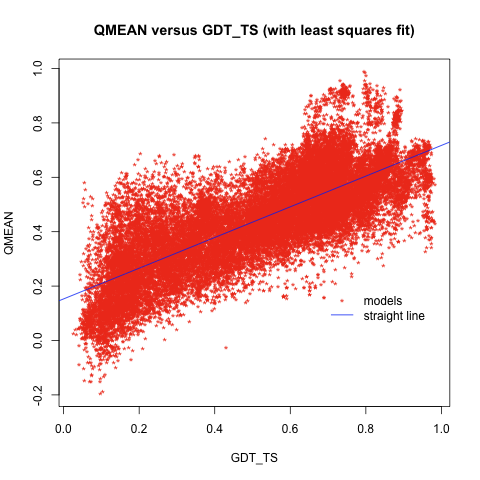
\includegraphics[scale=0.50]{casp8_QMEAN}
		\caption[QMEAN versus GDT\_TS on the CASP-8 test set]{QMEAN versus GDT\_TS on the CASP-8 test set. Globally, it presents the same accuracy for FM, TBM and HQM models.}
		\label{fig:casp8_qmean}
	\end{center}
\end{figure}

\begin{figure}[H]
	\begin{center}
		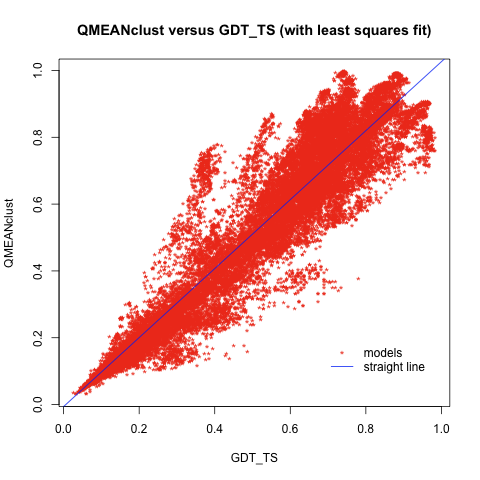
\includegraphics[scale=0.50]{casp8_QMEANclust}
		\caption[QMEANclust versus GDT\_TS on the CASP-8 test set]{QMEANclust versus GDT\_TS on the CASP-8 test set. It is the fourth best method concurring in CASP-8. It shows high accuracy for FM models, however does not assess exactly HQM model scores, leaving a hole in the high-right part of the scatter plot. Also many false positives and negatives are present in the center of the plot (TBM models).}
		\label{fig:casp8_qmeanclust}
	\end{center}
\end{figure}

\begin{figure}[H]
	\begin{center}
		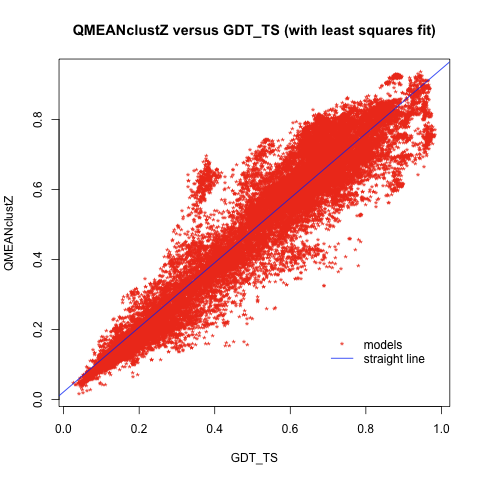
\includegraphics[scale=0.50]{casp8_QMEANclustZ}
		\caption[QMEANclustZ versus GDT\_TS on the CASP-8 test set]{QMEANclustZ versus GDT\_TS on the CASP-8 test set. This method improves QMEANclust by reducing the presence of false positives and negatives for TBM and HQM models. This plot cleanness is due to the presence of the feature $PFractionModelled$ that is able to lower incomplete model scores, but not so drastically as the pure $FractionModelled$ does. Also, it scores correctly HQM models.}
		\label{fig:casp8_qmeanclustZ}
	\end{center}
\end{figure}

\begin{figure}[H]
	\begin{center}
		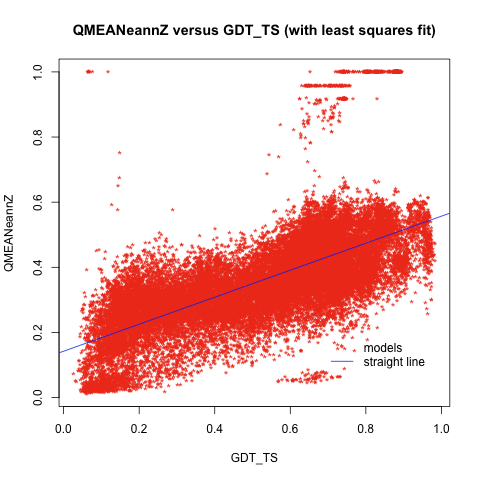
\includegraphics[scale=0.50]{casp8_std_G_medianQMEANeannZ}
		\caption[QMEANeannZ versus GDT\_TS on the CASP-8 test set, using Gauss integrals and fixed ANN architectures]{QMEANeannZ versus GDT\_TS on the CASP-8 test set, using Gauss integrals and fixed ANN architectures. This is the worst individual method. The predicted scores are very lower than the respective real scores, so the global Pearson correlation decreases with respect to that achieved by QMEAN. Methods using Gauss integrals are demonstrated to not be very reliable.}
		\label{fig:casp8_std_G_median_qmeaneannZ}
	\end{center}
\end{figure}

\begin{figure}[H]
	\begin{center}
		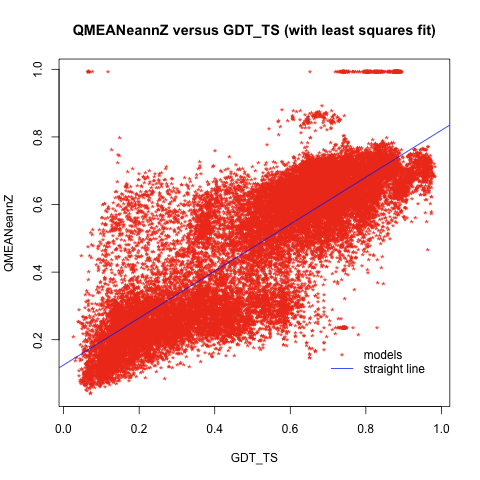
\includegraphics[scale=0.50]{casp8_std_H_medianQMEANeannZ}
		\caption[QMEANeannZ versus GDT\_TS on the CASP-8 test set, using hydrogen bonds and fixed ANN architectures]{QMEANeannZ versus GDT\_TS on the CASP-8 test set, using hydrogen bonds and fixed ANN architectures. A lot of false positives and negatives are present, however the two clouds are predicted correctly.}
		\label{fig:casp8_std_H_median_qmeaneannZ}
	\end{center}
\end{figure}

\begin{figure}[H]
	\begin{center}
		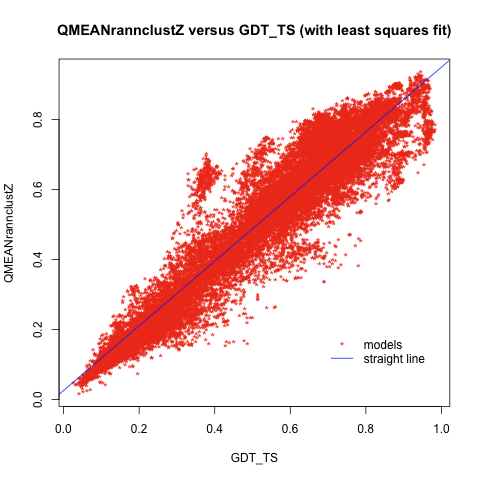
\includegraphics[scale=0.50]{casp8_std_H_medianQMEANrannclustZ}
		\caption[QMEANrannclustZ versus GDT\_TS on the CASP-8 test set, using hydrogen bonds and fixed ANN architecture]{QMEANrannclustZ versus GDT\_TS on the CASP-8 test set, using hydrogen bonds and fixed ANN architecture. This is the best clustering method presented with a Pearson correlation of $\approx 0.9485$. Only a little cloud of false positive is located in the center-left of the plot. Also HQM models are predicted correctly.}
		\label{fig:casp8_std_H_median_qmeanrannclustZ}
	\end{center}
\end{figure}

\begin{figure}[H]
	\begin{center}
		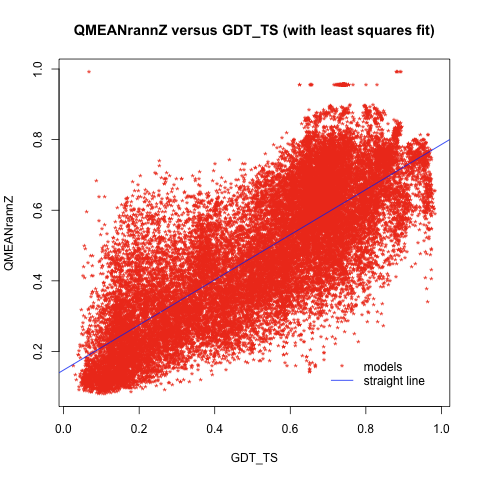
\includegraphics[scale=0.50]{casp8_std_medianQMEANrannZ}
		\caption[QMEANrannZ versus GDT\_TS on the CASP-8 test set using fixed ANN architecture]{QMEANrannZ versus GDT\_TS on the CASP-8 test set using fixed ANN architectures.}
		\label{fig:casp8_std_median_qmeanrannZ}
	\end{center}
\end{figure}

\begin{figure}[H]
	\begin{center}
		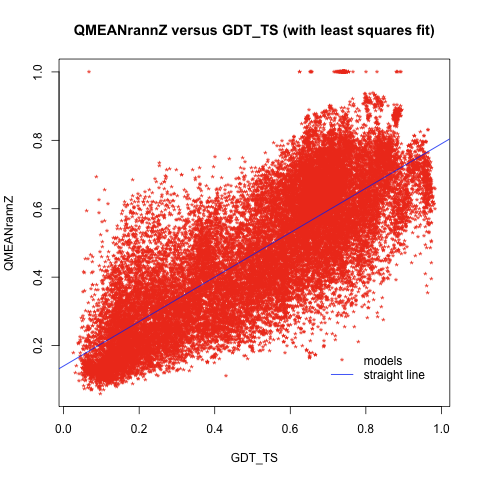
\includegraphics[scale=0.50]{casp8_cascade_std_medianQMEANrannZ}
		\caption[QMEANrannZ versus GDT\_TS on the CASP-8 test set, using ca\-sca\-de-\-cor\-re\-la\-tion ANN architecture]{QMEANrannZ versus GDT\_TS on the CASP-8 test set, using ca\-sca\-de-\-cor\-re\-la\-tion ANN architecture.}
		\label{fig:casp8_cascade_std_median_qmeanrannZ}
	\end{center}
\end{figure}

\begin{figure}[H]
	\begin{center}
		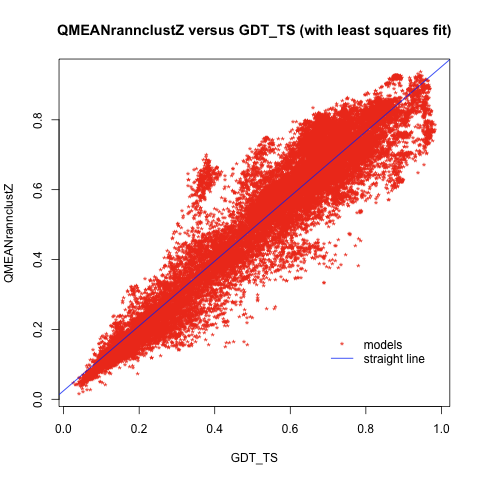
\includegraphics[scale=0.50]{casp8_cascade_std_medianQMEANrannclustZ}
		\caption[QMEANrannclustZ versus GDT\_TS on the CASP-8 test set, using ca\-sca\-de-\-cor\-re\-la\-tion ANN architecture]{QMEANrannclustZ versus GDT\_TS on the CASP-8 test set, using ca\-sca\-de-\-cor\-re\-la\-tion ANN architecture.}
		\label{fig:casp8_cascade_std_median_qmeanrannclustZ}
	\end{center}
\end{figure}

\begin{figure}[H]
	\begin{center}
		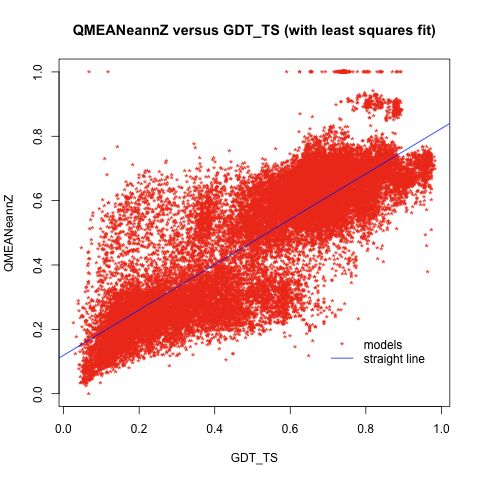
\includegraphics[scale=0.50]{casp8_cascade_std_H_medianQMEANeannZ}
		\caption[QMEANeannZ versus GDT\_TS on the CASP-8 test set, using hydrogen bonds and ca\-sca\-de-\-cor\-re\-la\-tion ANN architectures]{QMEANeannZ versus GDT\_TS on the CASP-8 test set, using hydrogen bonds and ca\-sca\-de-\-cor\-re\-la\-tion ANN architectures.}
		\label{fig:casp8_cascade_std_H_median_qmeaneannZ}
	\end{center}
\end{figure}

\begin{figure}[H]
	\begin{center}
		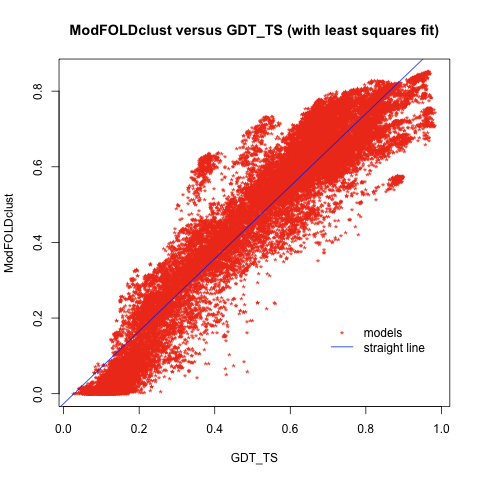
\includegraphics[scale=0.50]{casp8_ModFOLDclust}
		\caption[ModFOLDclust versus GDT\_TS on the CASP-8 test set]{ModFOLDclust versus GDT\_TS on the CASP-8 test set. This is the best method participating in CASP-8. The scatter plot present only some false negative. The cloud of false positive at coordinate $(0.4, 0.6)$ is common to all method predictions. That suggests a singular difficult target to predict.}
		\label{fig:casp8_modfoldclust}
	\end{center}
\end{figure}

\begin{figure}[H]
	\begin{center}
		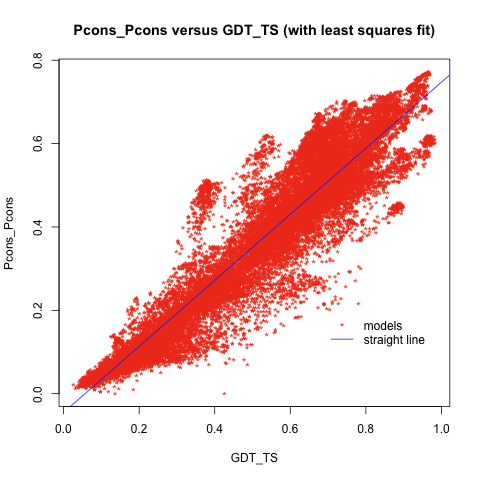
\includegraphics[scale=0.50]{casp8_Pcons_Pcons}
		\caption[Pcons\_Pcons versus GDT\_TS on the CASP-8 test set]{Pcons\_Pcons versus GDT\_TS on the CASP-8 test set. This is the second best method participating in CASP-8. It presents many false negative and does not predict correctly any HQM models.}
		\label{fig:casp8_pcons_pcons}
	\end{center}
\end{figure}

\begin{figure}[H]
	\begin{center}
		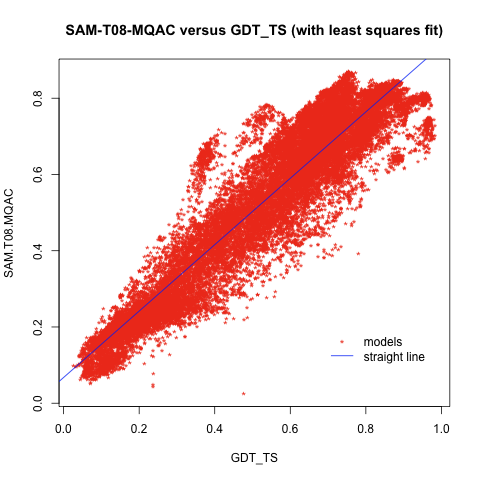
\includegraphics[scale=0.50]{casp8_SAM-T08-MQAC}
		\caption[SAM-T08-MQAC versus GDT\_TS on the CASP-8 test set]{SAM-T08-MQAC versus GDT\_TS on the CASP-8 test set. This is the third best method participating in CASP-8. The correlation is linear and well formed. However there is not high accuracy for FM models}
		\label{fig:casp8_sam-t08-mqac}
	\end{center}
\end{figure}






\cleardoublepage
